\documentclass{standalone}
\usepackage{tikz}
\usetikzlibrary{patterns, positioning}

\begin{document}
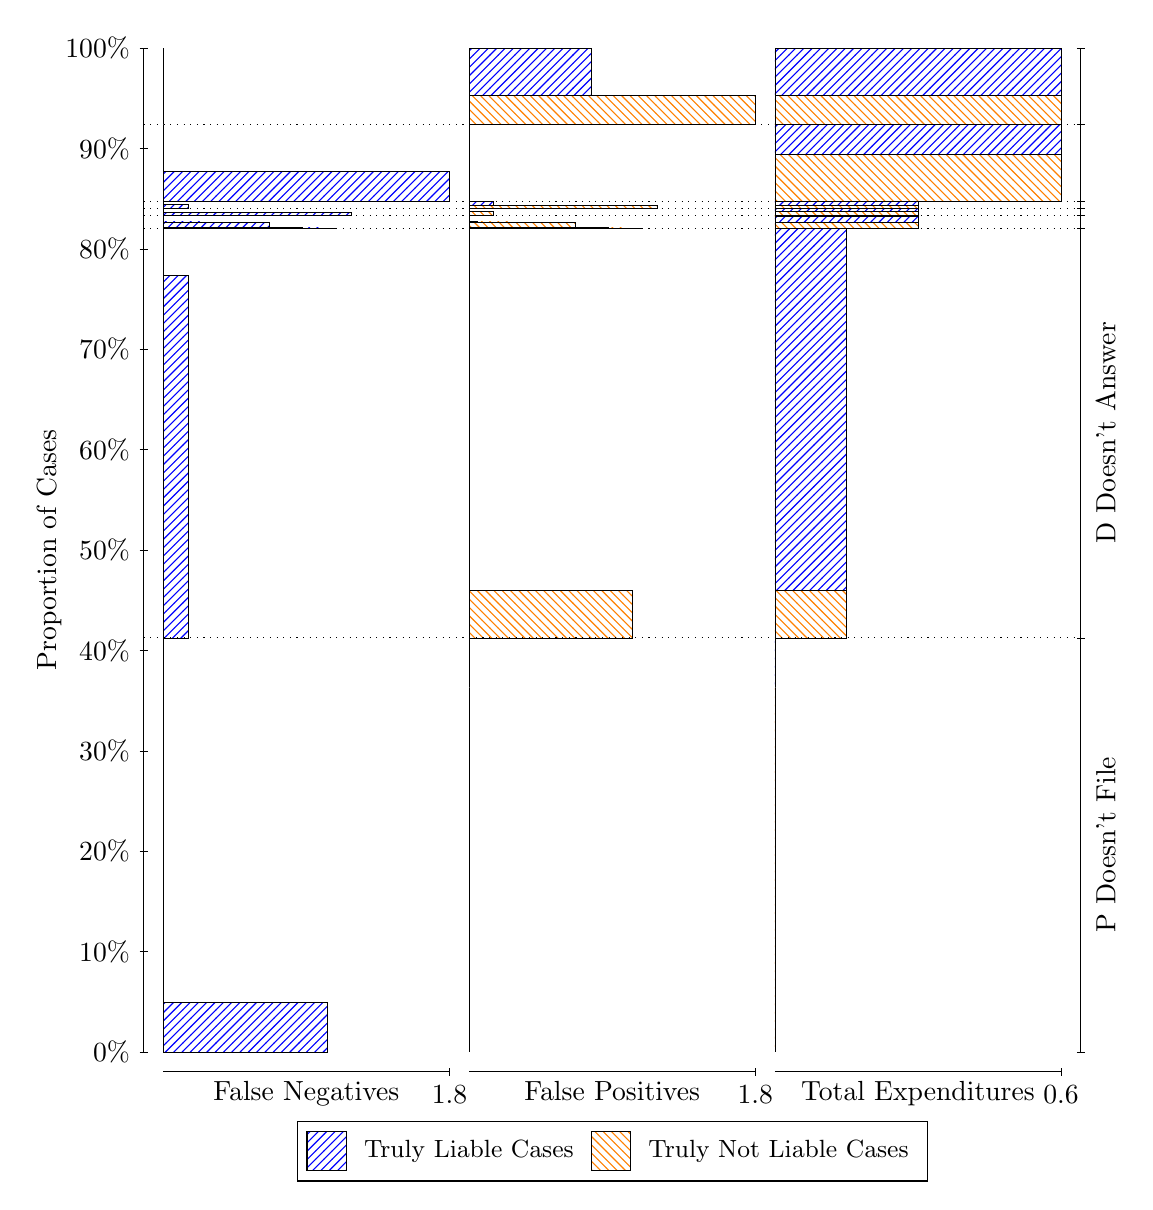
\begin{tikzpicture}
\draw[black, very thin] (1.5,1.75) -- (1.5,14.5);
\node[rotate=90, anchor=center] at (0.3, 8.125) {Proportion of Cases};
\draw[black, very thin] (1.45,1.75) -- (1.55,1.75);
\node[anchor=east] at (1.45, 1.75) {0\%};
\draw[black, very thin] (1.45,3.025) -- (1.55,3.025);
\node[anchor=east] at (1.45, 3.025) {10\%};
\draw[black, very thin] (1.45,4.3) -- (1.55,4.3);
\node[anchor=east] at (1.45, 4.3) {20\%};
\draw[black, very thin] (1.45,5.575) -- (1.55,5.575);
\node[anchor=east] at (1.45, 5.575) {30\%};
\draw[black, very thin] (1.45,6.85) -- (1.55,6.85);
\node[anchor=east] at (1.45, 6.85) {40\%};
\draw[black, very thin] (1.45,8.125) -- (1.55,8.125);
\node[anchor=east] at (1.45, 8.125) {50\%};
\draw[black, very thin] (1.45,9.4) -- (1.55,9.4);
\node[anchor=east] at (1.45, 9.4) {60\%};
\draw[black, very thin] (1.45,10.675) -- (1.55,10.675);
\node[anchor=east] at (1.45, 10.675) {70\%};
\draw[black, very thin] (1.45,11.95) -- (1.55,11.95);
\node[anchor=east] at (1.45, 11.95) {80\%};
\draw[black, very thin] (1.45,13.225) -- (1.55,13.225);
\node[anchor=east] at (1.45, 13.225) {90\%};
\draw[black, very thin] (1.45,14.5) -- (1.55,14.5);
\node[anchor=east] at (1.45, 14.5) {100\%};

\draw[black, very thin] (13.4,1.75) -- (13.4,14.5);
\draw[black, very thin] (13.35,1.75) -- (13.45,1.75);
\node[anchor=west] at (13.35, 1.75) {};
\draw[black, very thin] (13.35,7.01) -- (13.45,7.01);
\node[anchor=west] at (13.35, 7.01) {};
\draw[black, very thin] (13.35,12.211) -- (13.45,12.211);
\node[anchor=west] at (13.35, 12.211) {};
\draw[black, very thin] (13.35,12.373) -- (13.45,12.373);
\node[anchor=west] at (13.35, 12.373) {};
\draw[black, very thin] (13.35,12.465) -- (13.45,12.465);
\node[anchor=west] at (13.35, 12.465) {};
\draw[black, very thin] (13.35,12.556) -- (13.45,12.556);
\node[anchor=west] at (13.35, 12.556) {};
\draw[black, very thin] (13.35,13.528) -- (13.45,13.528);
\node[anchor=west] at (13.35, 13.528) {};
\draw[black, very thin] (13.35,14.5) -- (13.45,14.5);
\node[anchor=west] at (13.35, 14.5) {};

\draw[black, very thin, pattern color=blue, pattern=north east lines] (1.75,1.75) rectangle (3.8262,2.3828);
\draw[black, very thin, pattern color=orange, pattern=north west lines] (1.75,2.3828) rectangle (1.75,7.01);
\draw[black, very thin, pattern color=blue, pattern=north east lines] (1.75,7.01) rectangle (2.0614,11.608);
\draw[black, very thin, pattern color=orange, pattern=north west lines] (1.75,11.608) rectangle (1.75,12.211);
\draw[black, very thin, pattern color=blue, pattern=north east lines] (1.75,12.211) rectangle (3.93,12.214);
\draw[black, very thin, pattern color=blue, pattern=north east lines] (1.75,12.214) rectangle (3.7224,12.215);
\draw[black, very thin, pattern color=blue, pattern=north east lines] (1.75,12.215) rectangle (3.5148,12.218);
\draw[black, very thin, pattern color=blue, pattern=north east lines] (1.75,12.218) rectangle (3.3071,12.22);
\draw[black, very thin, pattern color=blue, pattern=north east lines] (1.75,12.22) rectangle (3.0995,12.281);
\draw[black, very thin, pattern color=blue, pattern=north east lines] (1.75,12.281) rectangle (2.8919,12.283);
\draw[black, very thin, pattern color=blue, pattern=north east lines] (1.75,12.283) rectangle (2.6843,12.286);
\draw[black, very thin, pattern color=blue, pattern=north east lines] (1.75,12.286) rectangle (2.4767,12.287);
\draw[black, very thin, pattern color=blue, pattern=north east lines] (1.75,12.287) rectangle (2.269,12.292);
\draw[black, very thin, pattern color=orange, pattern=north west lines] (1.75,12.292) rectangle (1.75,12.373);
\draw[black, very thin, pattern color=blue, pattern=north east lines] (1.75,12.373) rectangle (4.1376,12.411);
\draw[black, very thin, pattern color=orange, pattern=north west lines] (1.75,12.411) rectangle (1.75,12.465);
\draw[black, very thin, pattern color=blue, pattern=north east lines] (1.75,12.465) rectangle (2.0614,12.518);
\draw[black, very thin, pattern color=orange, pattern=north west lines] (1.75,12.518) rectangle (1.75,12.556);
\draw[black, very thin, pattern color=blue, pattern=north east lines] (1.75,12.556) rectangle (5.3833,12.931);
\draw[black, very thin, pattern color=orange, pattern=north west lines] (1.75,12.931) rectangle (1.75,13.528);
\draw[black, very thin, pattern color=orange, pattern=north west lines] (1.75,13.528) rectangle (1.75,13.903);
\draw[black, very thin, pattern color=blue, pattern=north east lines] (1.75,13.903) rectangle (1.75,14.5);
\draw[black, very thin, pattern color=orange, pattern=north west lines] (5.6333,1.75) rectangle (5.6333,6.3773);
\draw[black, very thin, pattern color=blue, pattern=north east lines] (5.6333,6.3773) rectangle (5.6333,7.01);
\draw[black, very thin, pattern color=orange, pattern=north west lines] (5.6333,7.01) rectangle (7.7095,7.6132);
\draw[black, very thin, pattern color=blue, pattern=north east lines] (5.6333,7.6132) rectangle (5.6333,12.211);
\draw[black, very thin, pattern color=orange, pattern=north west lines] (5.6333,12.211) rectangle (7.8133,12.214);
\draw[black, very thin, pattern color=orange, pattern=north west lines] (5.6333,12.214) rectangle (7.6057,12.215);
\draw[black, very thin, pattern color=orange, pattern=north west lines] (5.6333,12.215) rectangle (7.3981,12.218);
\draw[black, very thin, pattern color=orange, pattern=north west lines] (5.6333,12.218) rectangle (7.1905,12.22);
\draw[black, very thin, pattern color=orange, pattern=north west lines] (5.6333,12.22) rectangle (6.9829,12.281);
\draw[black, very thin, pattern color=orange, pattern=north west lines] (5.6333,12.281) rectangle (6.7752,12.283);
\draw[black, very thin, pattern color=orange, pattern=north west lines] (5.6333,12.283) rectangle (6.7752,12.283);
\draw[black, very thin, pattern color=orange, pattern=north west lines] (5.6333,12.283) rectangle (6.5676,12.286);
\draw[black, very thin, pattern color=orange, pattern=north west lines] (5.6333,12.286) rectangle (6.36,12.287);
\draw[black, very thin, pattern color=orange, pattern=north west lines] (5.6333,12.287) rectangle (6.1524,12.292);
\draw[black, very thin, pattern color=blue, pattern=north east lines] (5.6333,12.292) rectangle (5.7371,12.296);
\draw[black, very thin, pattern color=blue, pattern=north east lines] (5.6333,12.296) rectangle (5.6333,12.373);
\draw[black, very thin, pattern color=orange, pattern=north west lines] (5.6333,12.373) rectangle (5.9448,12.427);
\draw[black, very thin, pattern color=blue, pattern=north east lines] (5.6333,12.427) rectangle (5.6333,12.465);
\draw[black, very thin, pattern color=orange, pattern=north west lines] (5.6333,12.465) rectangle (8.021,12.503);
\draw[black, very thin, pattern color=blue, pattern=north east lines] (5.6333,12.503) rectangle (5.9448,12.556);
\draw[black, very thin, pattern color=orange, pattern=north west lines] (5.6333,12.556) rectangle (5.6333,13.153);
\draw[black, very thin, pattern color=blue, pattern=north east lines] (5.6333,13.153) rectangle (5.6333,13.528);
\draw[black, very thin, pattern color=orange, pattern=north west lines] (5.6333,13.528) rectangle (9.2667,13.903);
\draw[black, very thin, pattern color=blue, pattern=north east lines] (5.6333,13.903) rectangle (7.1905,14.5);
\draw[black, very thin, pattern color=orange, pattern=north west lines] (9.5167,1.75) rectangle (9.5167,6.3773);
\draw[black, very thin, pattern color=blue, pattern=north east lines] (9.5167,6.3773) rectangle (9.5167,7.01);
\draw[black, very thin, pattern color=orange, pattern=north west lines] (9.5167,7.01) rectangle (10.425,7.6132);
\draw[black, very thin, pattern color=blue, pattern=north east lines] (9.5167,7.6132) rectangle (10.425,12.211);
\draw[black, very thin, pattern color=orange, pattern=north west lines] (9.5167,12.211) rectangle (11.333,12.283);
\draw[black, very thin, pattern color=blue, pattern=north east lines] (9.5167,12.283) rectangle (11.333,12.357);
\draw[black, very thin, pattern color=orange, pattern=north west lines] (9.5167,12.357) rectangle (11.333,12.362);
\draw[black, very thin, pattern color=blue, pattern=north east lines] (9.5167,12.362) rectangle (11.333,12.365);
\draw[black, very thin, pattern color=orange, pattern=north west lines] (9.5167,12.365) rectangle (11.333,12.369);
\draw[black, very thin, pattern color=blue, pattern=north east lines] (9.5167,12.369) rectangle (11.333,12.373);
\draw[black, very thin, pattern color=orange, pattern=north west lines] (9.5167,12.373) rectangle (11.333,12.427);
\draw[black, very thin, pattern color=blue, pattern=north east lines] (9.5167,12.427) rectangle (11.333,12.465);
\draw[black, very thin, pattern color=orange, pattern=north west lines] (9.5167,12.465) rectangle (11.333,12.503);
\draw[black, very thin, pattern color=blue, pattern=north east lines] (9.5167,12.503) rectangle (11.333,12.556);
\draw[black, very thin, pattern color=orange, pattern=north west lines] (9.5167,12.556) rectangle (13.15,13.153);
\draw[black, very thin, pattern color=blue, pattern=north east lines] (9.5167,13.153) rectangle (13.15,13.528);
\draw[black, very thin, pattern color=orange, pattern=north west lines] (9.5167,13.528) rectangle (13.15,13.903);
\draw[black, very thin, pattern color=blue, pattern=north east lines] (9.5167,13.903) rectangle (13.15,14.5);
\draw[black, dotted] (1.5,7.01) -- (13.4,7.01);
\draw[black, dotted] (1.5,12.211) -- (13.4,12.211);
\draw[black, dotted] (1.5,12.373) -- (13.4,12.373);
\draw[black, dotted] (1.5,12.465) -- (13.4,12.465);
\draw[black, dotted] (1.5,12.556) -- (13.4,12.556);
\draw[black, dotted] (1.5,13.528) -- (13.4,13.528);
\draw[black, very thin] (1.75,1.5) -- (5.3833,1.5);
\node[anchor=north] at (3.5667, 1.5) {False Negatives};
\draw[black, very thin] (5.3833,1.45) -- (5.3833,1.55);
\node[anchor=north] at (5.3833, 1.45) {1.8};

\draw[black, very thin] (5.6333,1.5) -- (9.2667,1.5);
\node[anchor=north] at (7.45, 1.5) {False Positives};
\draw[black, very thin] (9.2667,1.45) -- (9.2667,1.55);
\node[anchor=north] at (9.2667, 1.45) {1.8};

\draw[black, very thin] (9.5167,1.5) -- (13.15,1.5);
\node[anchor=north] at (11.333, 1.5) {Total Expenditures};
\draw[black, very thin] (13.15,1.45) -- (13.15,1.55);
\node[anchor=north] at (13.15, 1.45) {0.6};

\node[black, centered, rotate=90] at (13.72, 4.38) {P Doesn't File};
\node[black, centered, rotate=90] at (13.72, 9.6105) {D Doesn't Answer};






\draw (7.449999999999999,1.5) node[draw=none] (baseCoordinate) {};
\begin{scope}[align=center]
        \matrix[scale=0.5, draw=black, below=0.5cm of baseCoordinate, nodes={draw}, column sep=0.1cm]{
            \node[rectangle, draw, minimum width=0.5cm, minimum height=0.5cm, pattern=north east lines, pattern color=blue] {}; &
            \node[draw=none, font=\small] (B) {Truly Liable Cases}; &
            \node[rectangle, draw, minimum width=0.5cm, minimum height=0.5cm, pattern=north west lines, pattern color=orange] {}; &
            \node[draw=none, font=\small] (B) {Truly Not Liable Cases}; \\
            };
\end{scope}

\end{tikzpicture}
\end{document}